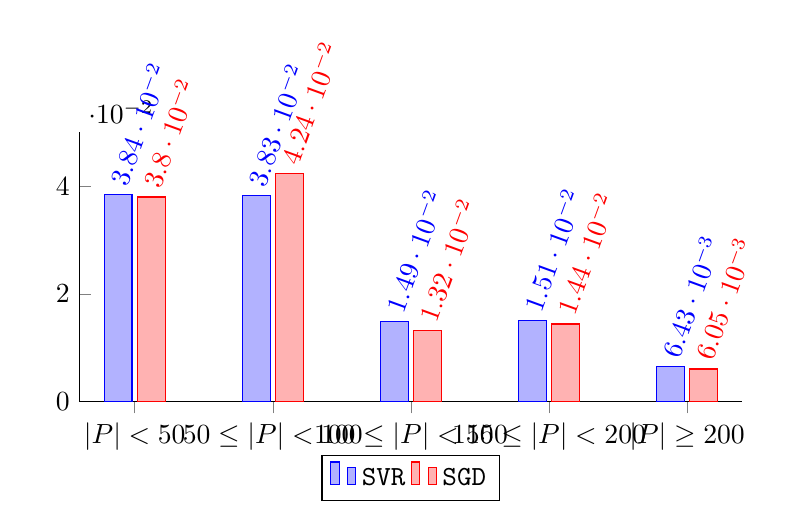
\begin{tikzpicture}
\begin{axis}[
	ybar,
	height=5cm,
	width=10cm,
	enlarge y limits=false,
	axis lines*=left,
	ymin=0,
	ymax=0.05,
	legend style={at={(0.5,-0.2)},
		anchor=north,legend columns=-1},
		ylabel={$\prerror$},
		symbolic x coords={50,100,150,200,201},
		xticklabels={
			$|P| < 50$,
			$50  \leq |P| < 100$,
			$100 \leq |P| < 150$,
			$150 \leq |P| < 200$,
			$|P| \geq 200$
		},
		xtick=data,
		nodes near coords,
		every node near coord/.append style={
			anchor=mid west,
			rotate=70
		}
	]
\addplot coordinates {
	(50,	0.0384)
	(100,	0.0383)
	(150,	0.0149)
	(200,	0.0151)
	(201,	0.00643)
};
\addplot coordinates {
	(50, 	0.0380)
	(100,	0.0424)
	(150,	0.0132)
	(200,	0.0144)
	(201,	0.00605)
};
\legend{\texttt{SVR},\texttt{SGD}}
\end{axis}
\end{tikzpicture}
